\documentclass[12pt]{article}

\usepackage{answers}
\usepackage{setspace}
\usepackage{graphicx}
\usepackage{enumitem}
\usepackage{multicol}
\usepackage{mathrsfs}
\usepackage[margin=1in]{geometry} 
\usepackage{amsmath,amsthm,amssymb}
\usepackage[ngerman]{babel}

\newcommand{\N}{\mathbb{N}}
\newcommand{\Z}{\mathbb{Z}}
\newcommand{\C}{\mathbb{C}}
\newcommand{\R}{\mathbb{R}}

\DeclareMathOperator{\sech}{sech}
\DeclareMathOperator{\csch}{csch}

\newenvironment{theorem}[2][Theorem]{\begin{trivlist}
		\item[\hskip \labelsep {\bfseries #1}\hskip \labelsep {\bfseries #2.}]}{\end{trivlist}}
\newenvironment{definition}[2][Definition]{\begin{trivlist}
		\item[\hskip \labelsep {\bfseries #1}\hskip \labelsep {\bfseries #2.}]}{\end{trivlist}}
\newenvironment{proposition}[2][Proposition]{\begin{trivlist}
		\item[\hskip \labelsep {\bfseries #1}\hskip \labelsep {\bfseries #2.}]}{\end{trivlist}}
\newenvironment{lemma}[2][Lemma]{\begin{trivlist}
		\item[\hskip \labelsep {\bfseries #1}\hskip \labelsep {\bfseries #2.}]}{\end{trivlist}}
\newenvironment{exercise}[2][Exercise]{\begin{trivlist}
		\item[\hskip \labelsep {\bfseries #1}\hskip \labelsep {\bfseries #2.}]}{\end{trivlist}}
\newenvironment{solution}[2][Solution]{\begin{trivlist}
		\item[\hskip \labelsep {\bfseries #1}]}{\end{trivlist}}
\newenvironment{problem}[2][Problem]{\begin{trivlist}
		\item[\hskip \labelsep {\bfseries #1}\hskip \labelsep {\bfseries #2.}]}{\end{trivlist}}
\newenvironment{question}[2][Question]{\begin{trivlist}
		\item[\hskip \labelsep {\bfseries #1}\hskip \labelsep {\bfseries #2.}]}{\end{trivlist}}
\newenvironment{corollary}[2][Corollary]{\begin{trivlist}
		\item[\hskip \labelsep {\bfseries #1}\hskip \labelsep {\bfseries #2.}]}{\end{trivlist}}

\begin{document}
	\title{Programmieren mit Neuronalen Netzen}
	\author{Michael Gabler}
	\maketitle
	\tableofcontents
	\newpage

	\section{Grundlagen}
	Neuronales Netzwerk ist Funktion, die auf Eingabedaten angewendet wird.\\
	\textbf{Optimierung} durch Minimierung der Loss-Funktion\\
	\textbf{Loss-Funktion} Maß, wie gut das Netzwerk Vorhersagen trifft. Berechnet sich aus Vorhersage und tatsächlichen Werten (Ground Truth).
	\begin{itemize}
		\item Euklidischer Loss, Mean-Squared-Error: $l_2 = \frac{1}{2N} \sum_i (f_\theta(x_i)-t_i)^2$
		\item Negative-Log-Likelihood, Cross-Entropy: $NLL = -\frac{1}{|D|}\sum_i \log[f_\theta(x_i)|_{t_i}]$
	\end{itemize}
	\textbf{Konfusionsmatrix} welche Klassen werden wie oft mit welcher Klasse verwechselt?\\
	\textbf{Linearisiertes Speichern mehrdimensionaler Objekte}\\
	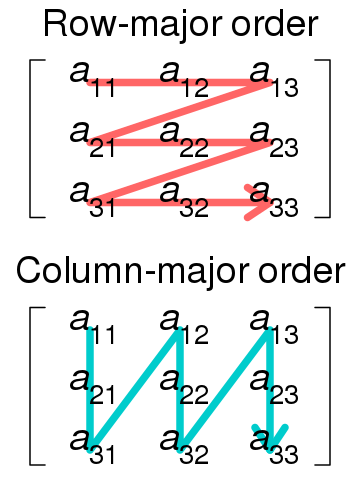
\includegraphics[width=0.25\linewidth]{figures/row-column-major.png}\\

	
	\subsection{Training}
	Daten werden aufgeteilt in Train/Validierung/Test (z.B. 60/20/20)\\
	\textbf{Datenaugmentierung} Generieren zusätzlicher Daten (z.B. bei Bildern) durch Spiegelung, Rotation, Skalierung, Anpassung Helligkeit und Farbe, etc.\\
	\textbf{Epoche} Verarbeitung aller Trainingsdaten\\
	\textbf{Iteration} Verarbeitung eines Batches\\
	\textbf{Batch} Mehrere Trainingsbeispiele werden gerechnet bevor Gewichte einmal geupdated werden (z.B. 10 Beispiele pro Batch)\\
	\textbf{Learning Rate} Faktor $\eta$, wie stark das Netzwerk durch die Deltas verändert werden soll (d.h. wie schnell es lernt bzw. seine Meinung ändert). Wird beim Update der Gewichte verwendet.
	\textbf{Evaluation auf Validierungsdaten} zur Anpassung der Hyperparameter (Learning-Rate, Netzstruktur, ...)\\
	\textbf{Evaluation auf Testdaten} einmalig, um Genauigkeit des trainierten Netzes zu ermitteln
	\textbf{Forward-Pass} Berechnen des Outputs des Netzwerkes für bestimmte Eingabedaten (z.B. ein Batch)\\
	\textbf{Backward-Pass} Bilden der partiellen Ableitung für jeden Input in jedem Layer und Speichern der Werte als Deltas\\
	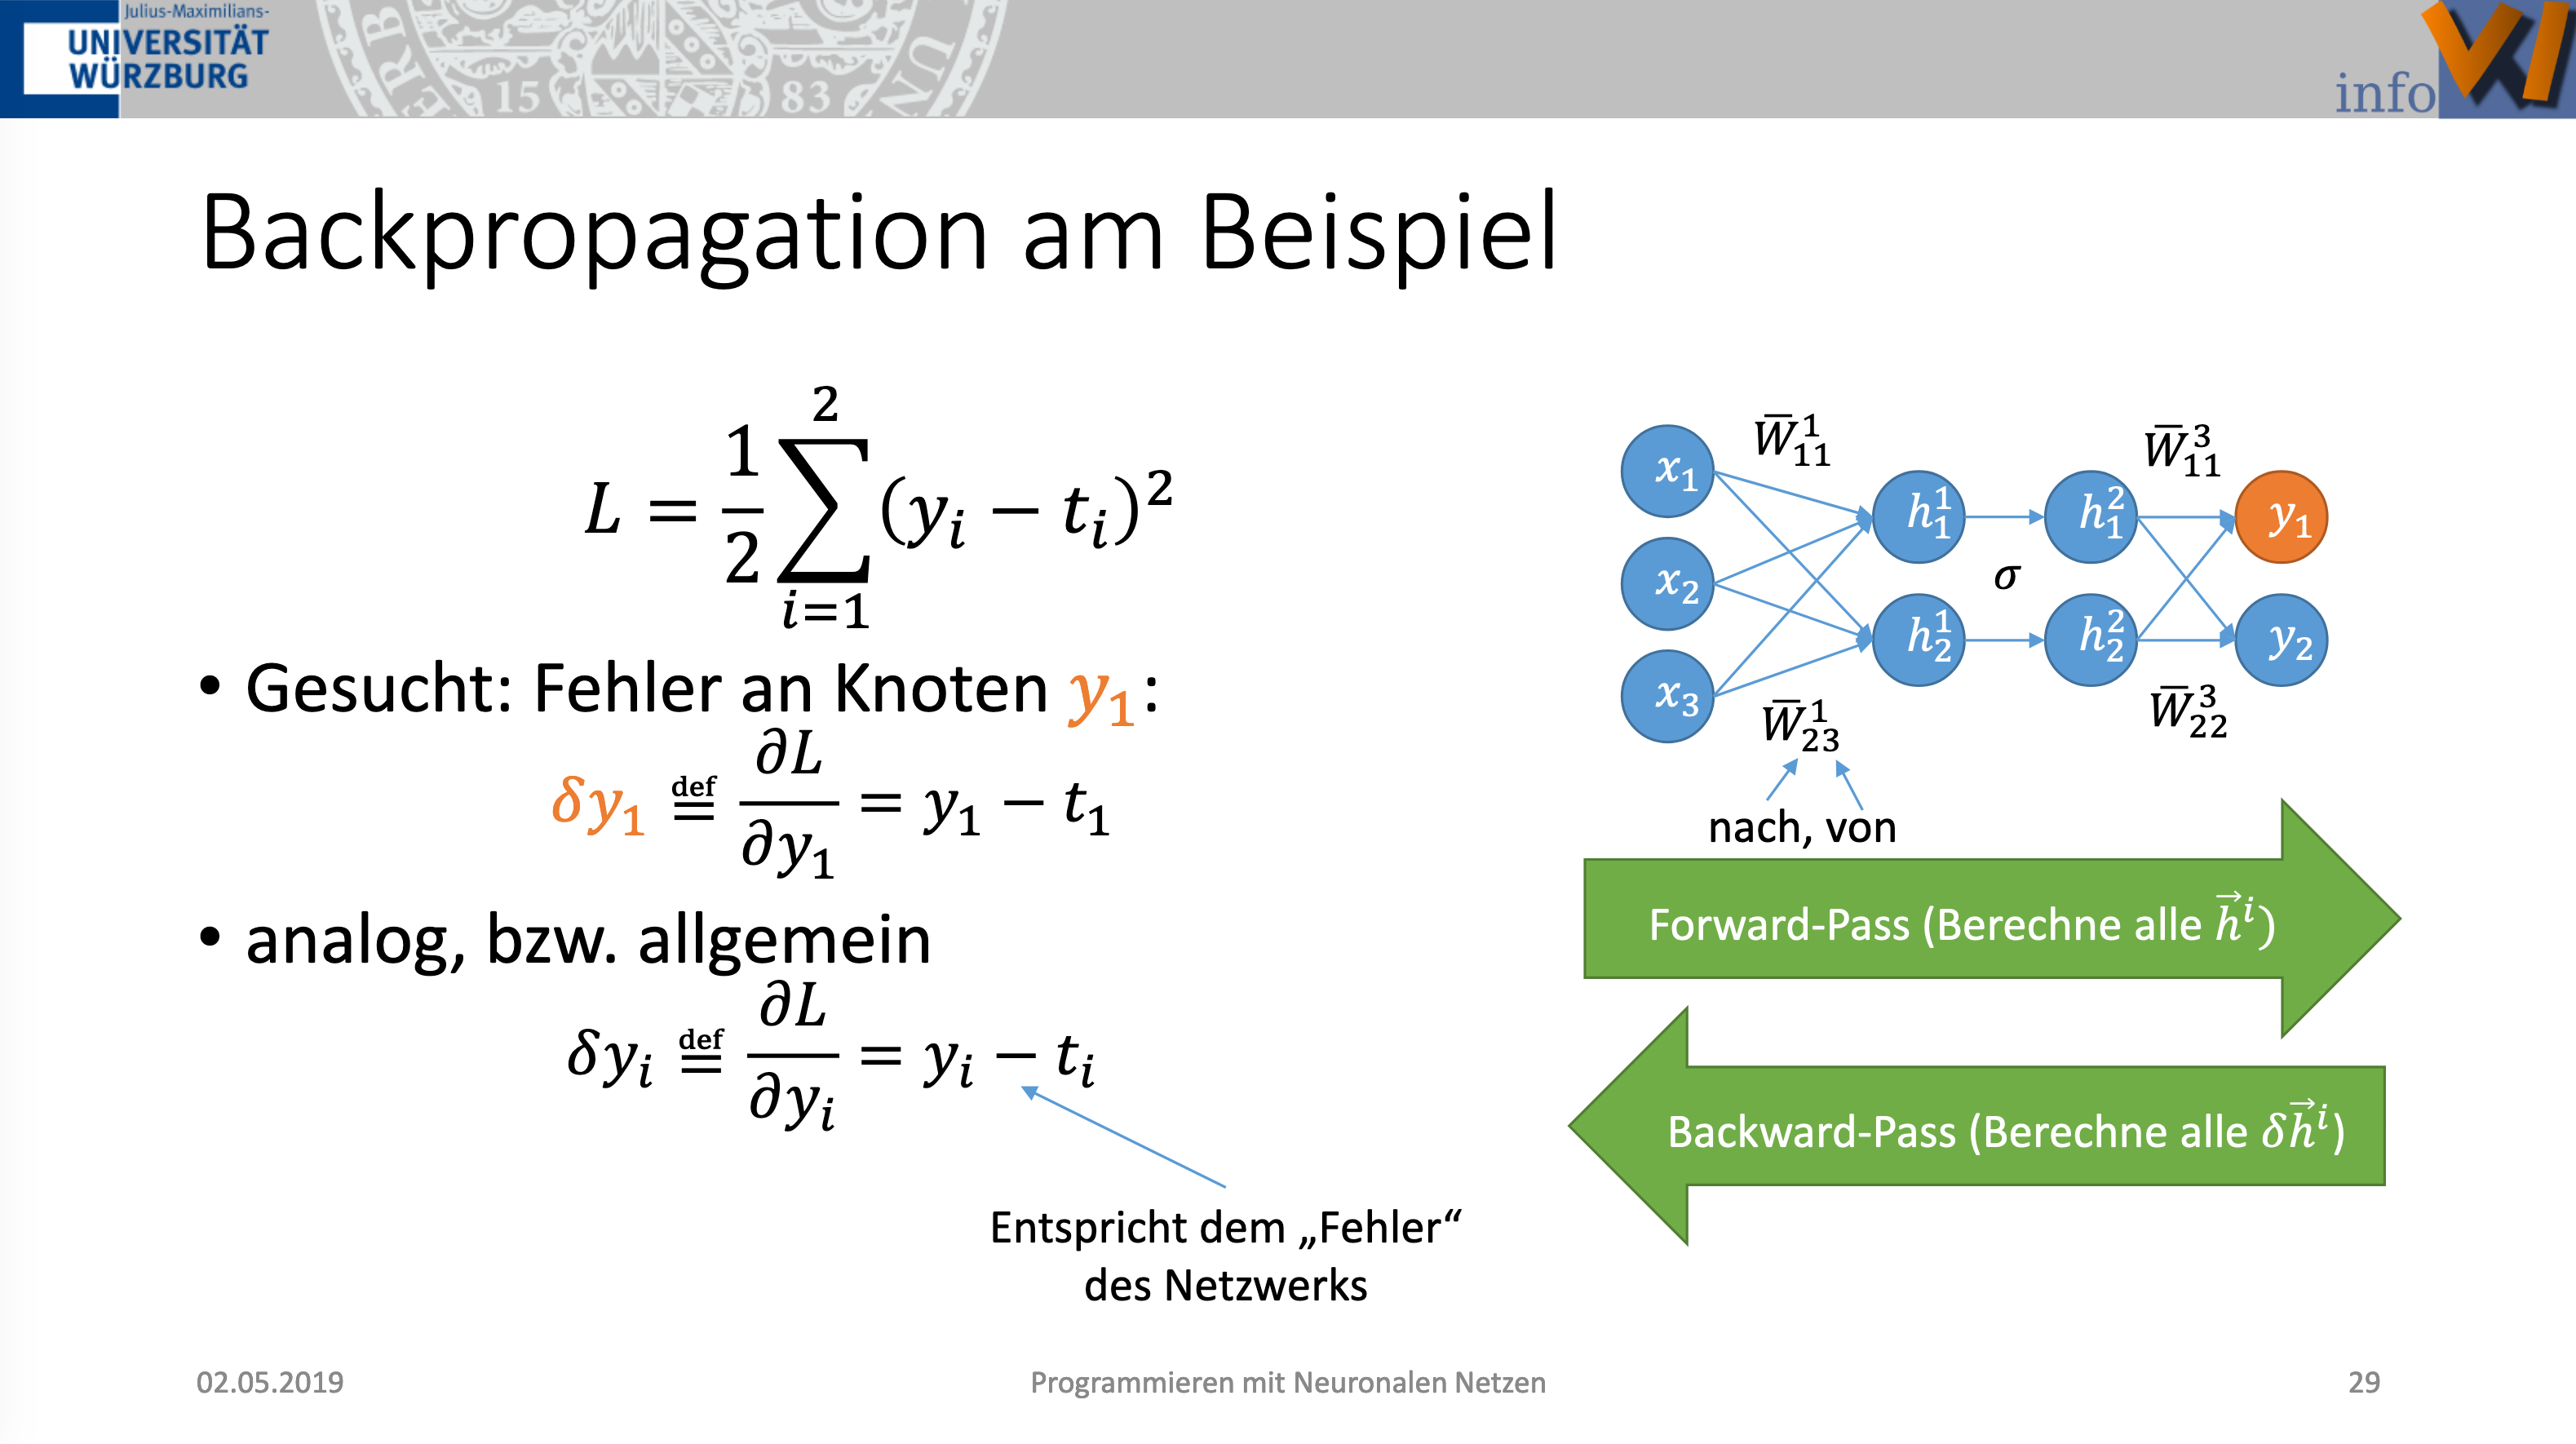
\includegraphics[width=\linewidth]{figures/backpropagation.png}\\
	\textbf{Berechnung der Gewicht-Deltas} Bilden der partiellen Ableitung für jedes Gewicht jedes Layers und Speichern der Werte als Deltas. Zur Berechnung sind die Deltas der Outputs (siehe Backward-Pass) erforderlich. Für Batches werden die Deltas der Gewichte aufsummiert und nach dem Batch geupdated.\\
	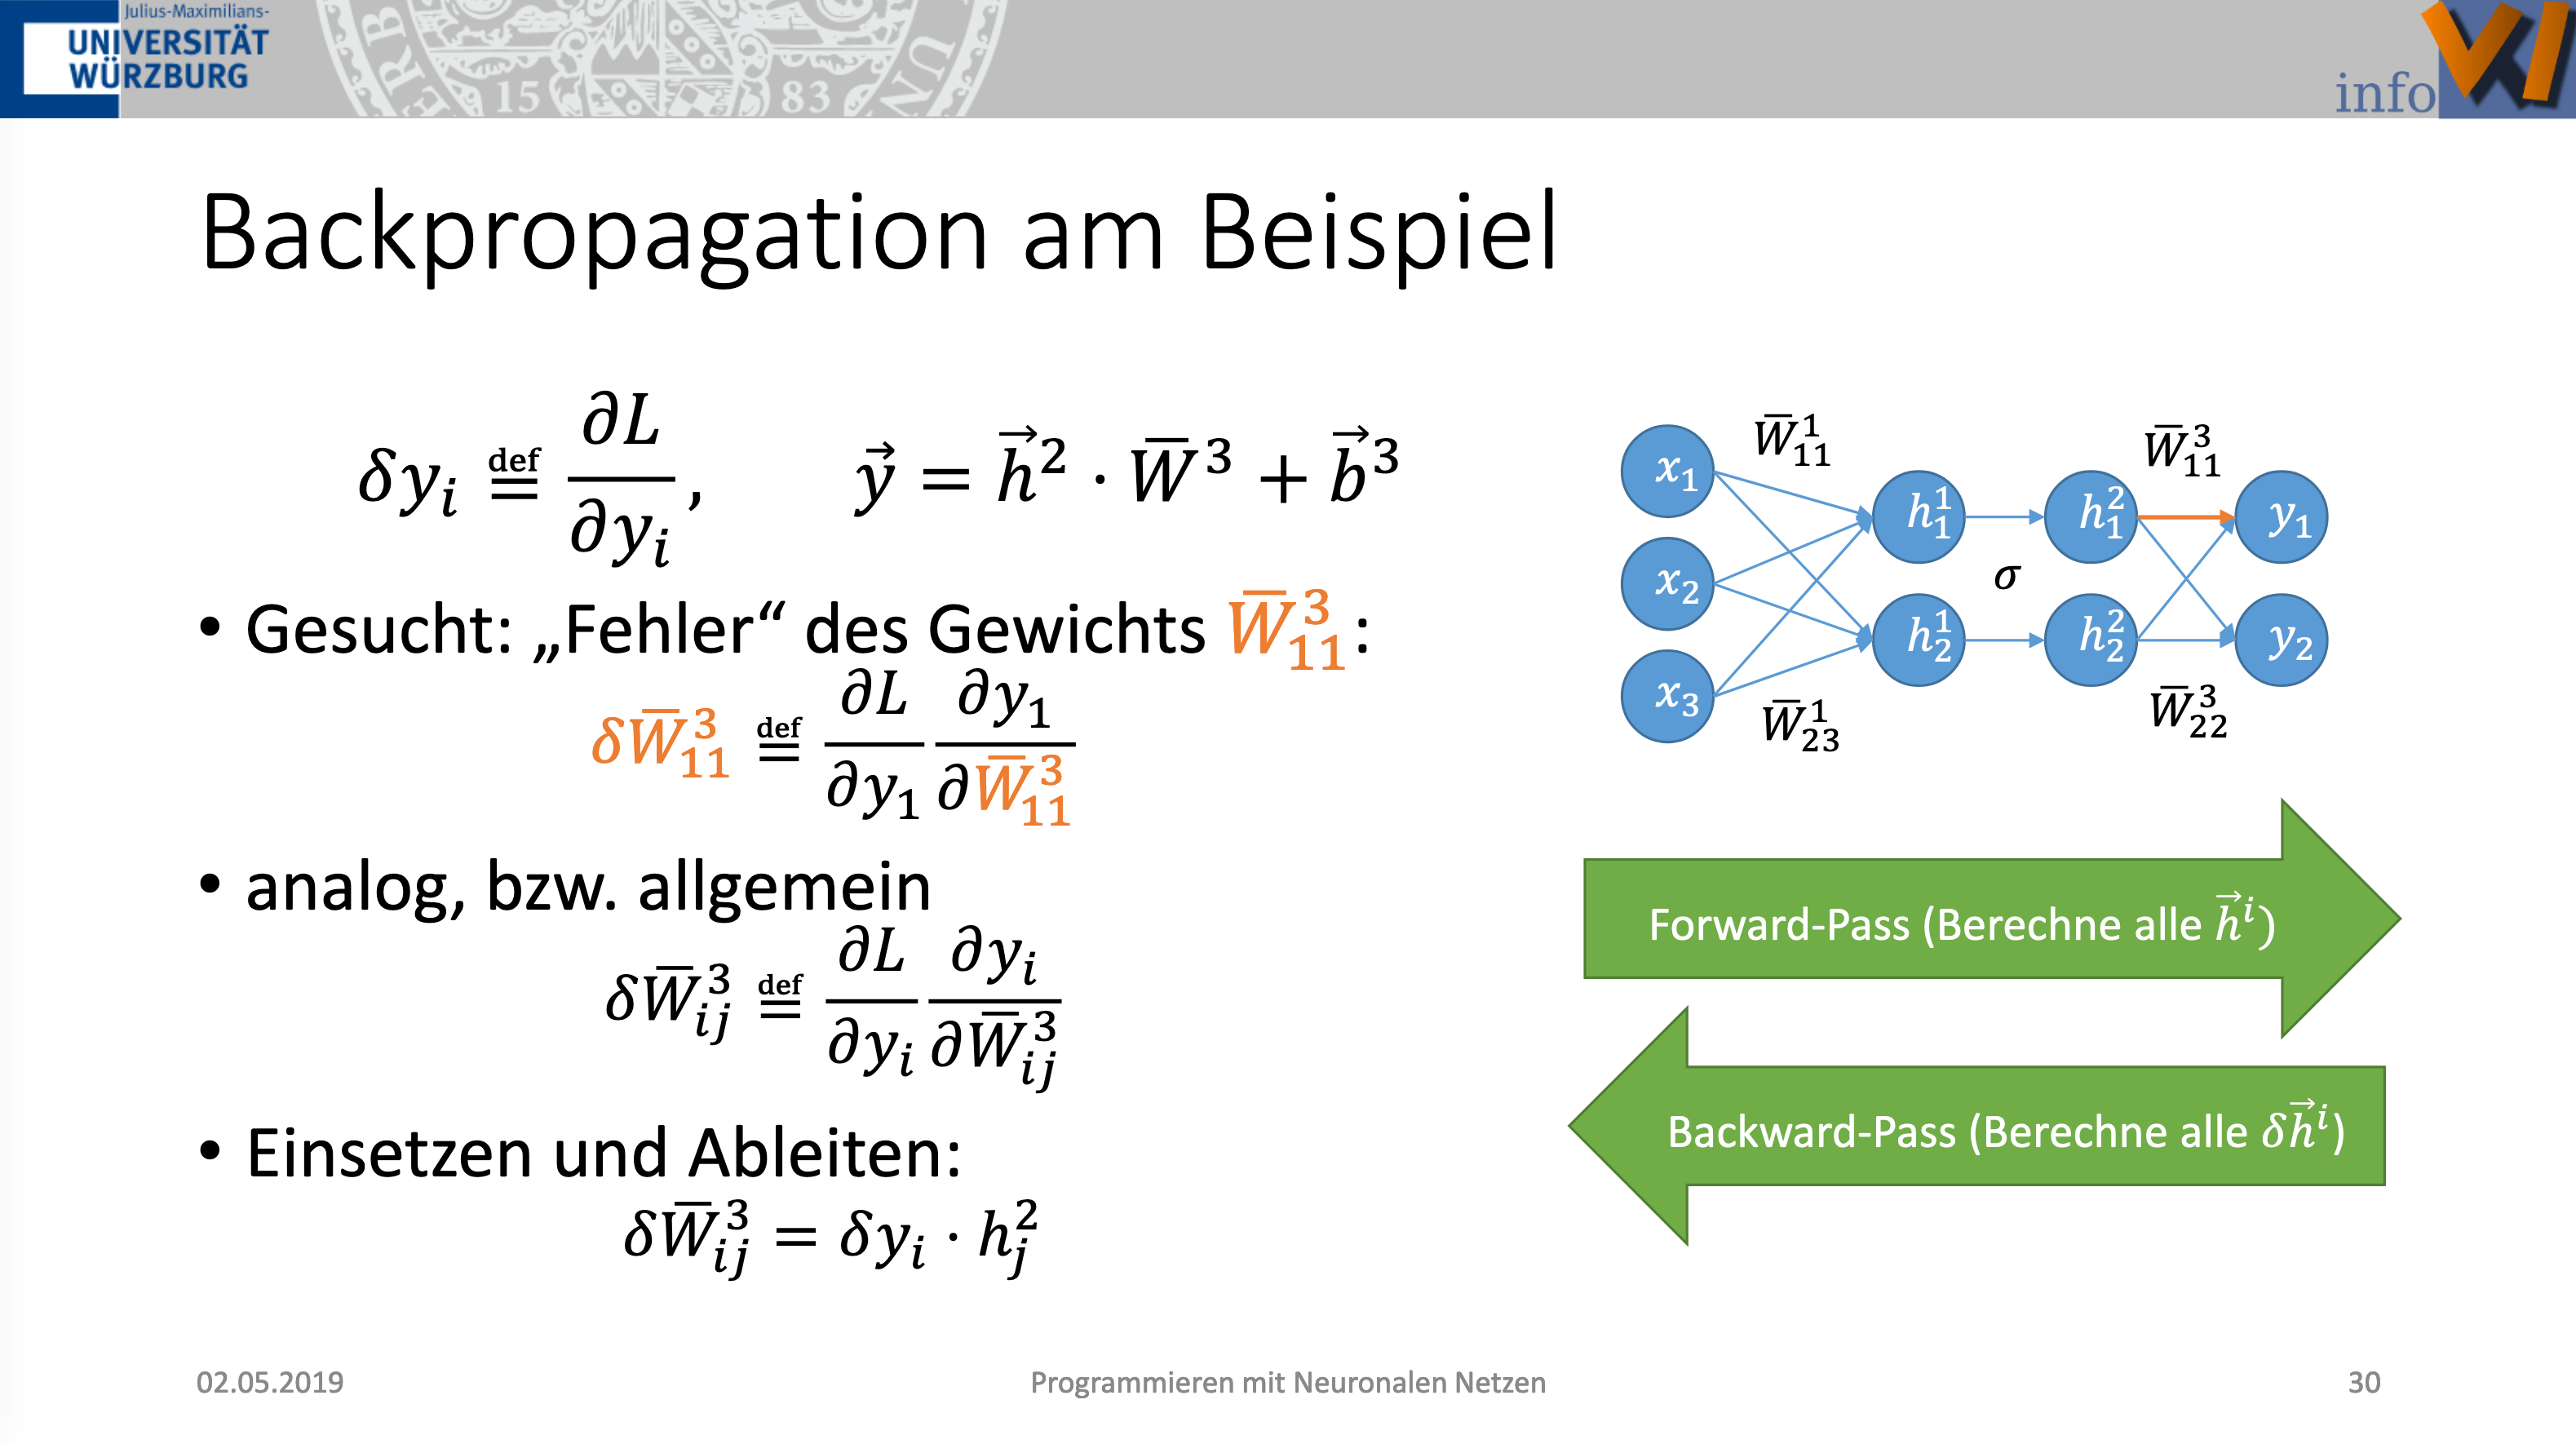
\includegraphics[width=\linewidth]{figures/calculate-delta-weights.png}\\
	\textbf{Update der Gewichte} Die Gewichte werden nun geupdated, in dem die Deltas der Gewichte mit den ursprünglichen Gewichten verrechnet werden. Dafür gibt es verschiedene Optimierungsverfahren:
	\begin{itemize}
		\item Gradient Descent: für Gewicht $w'_{ij} = w_{ij} - \eta \cdot \delta w_{ij}$
		\item Adam-Optimizer: robuster gegeüber schlecht gewählter Learning-Rate
		\item Adagrad
		\item RMSProp
	\end{itemize}
	\textbf{Regularisierung} Methoden um Overfitting vorzubeugen
	\begin{itemize}
		\item Rauschen auf Eingabedaten, Gewichten, Ausgabe (Zufallswerte hinzufügen)
		\item Datenaugmentierung
		\item Early-Stopping: Laufende Validierung auf Validierungsset, Trainingsabbruch wenn Accuracy abnimmt
		\item Dropout (siehe Layer)
		
	\end{itemize}
	\textbf{Pre-Training} Verwende Startgewichte, die bereits auf ähnlichen Daten trainiert wurden $\rightarrow$ besser als zufällige Initialisierung.\\
	\textbf{Transferlearning} Verwende vortrainiertes Netz und trainiere nur einzelne Schichten (z.B. letzte Schicht für Klassifikation) neu.

	\subsection{Netzarchitektur}
	\textbf{Perceptron} (= künstliches Neuron) stellt lineare Trennung (binäre Klassifikation) dar. Kann Funktionen AND, OR und NOT lernen, nicht aber XOR.\\
	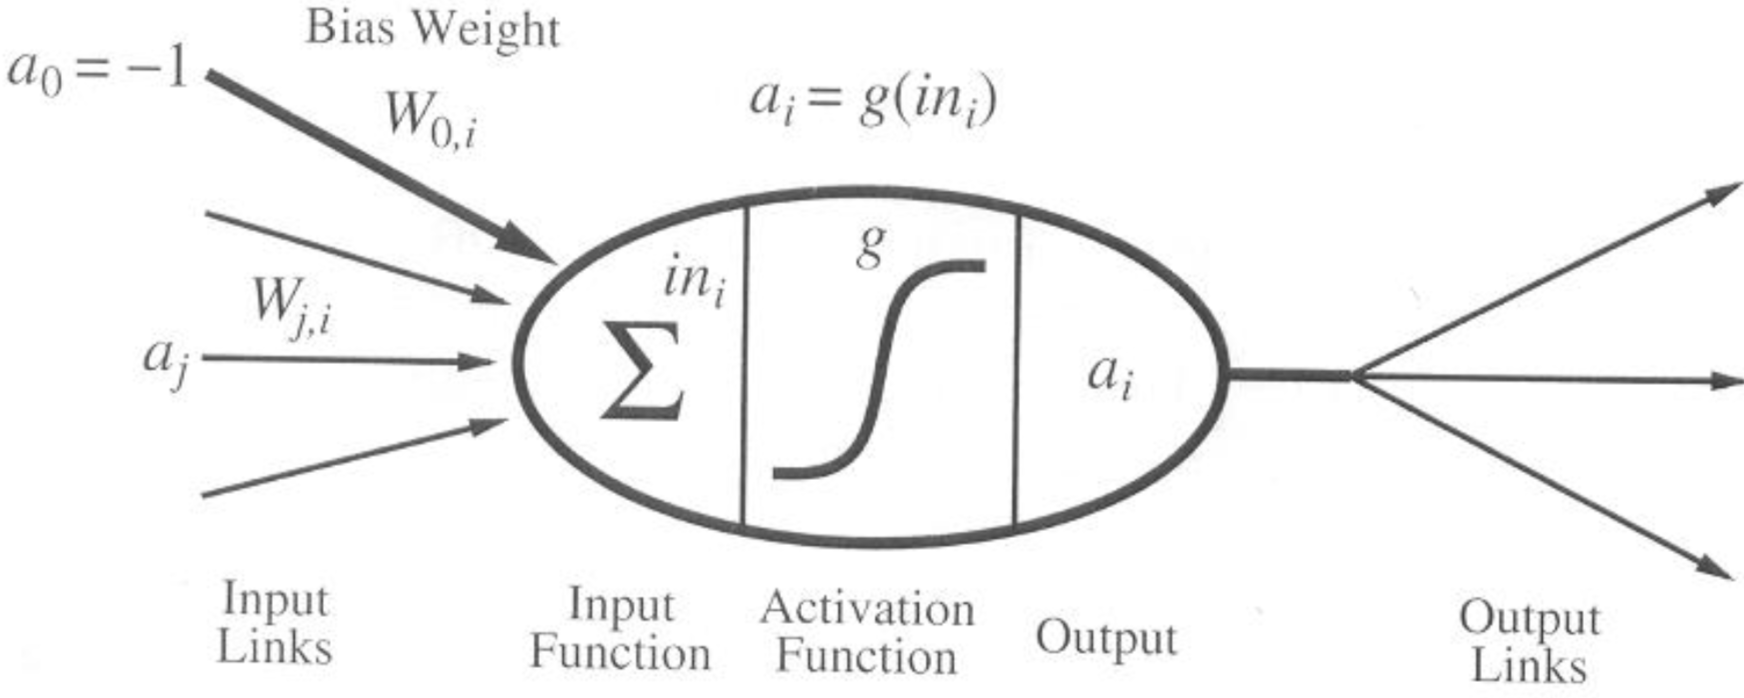
\includegraphics[width=\linewidth]{figures/perceptron.png}\\
	mit Inputs $a_j$ gewichtet mit $W_{ji}$ (ergeben zusammen die Gewichtsmatrix $W$), addiert mit Bias $b$, Outputs $a_i$ und der Aktivierungsfunktion $g$ mit der der Output berechnet wird.
	$$Ausgabe_{Schicht(x)} = g(Eingabe_{Schicht(x)} \cdot W + b) = Eingabe_{Schicht(x+1)}$$
	\textbf{Aktivierungsfunktion} muss bei Multi-Layer-Perceptronen (MLP) nicht-linear sein, da sonst nicht mehr Information gespeichert werden kann.
	$$(x \cdot W + b) \cdot V + a = x \cdot W \cdot V + b \cdot V + a = x \cdot W' + b'$$

	\section{Layer}
	Mögliche Schichten aus denen ein neuronales Netz bestehen kann.
	\subsection{Fully Connected / Dense}
	Voll verbundene Schicht, d.h. jeder Input landet in jedem Neuron. Wird z.B. als letzter Layer zur Klassifikation verwendet, um Vektor mit Logits für Klassen auszugeben.\\
	\textbf{Parameter} $X \in \R^{1 \times a}$: Eingabe, $W \in \R^{a \times n}$: Gewichtsmatrix, $b \in \R^{1 \times n}$: Bias, $n$: Anzahl der Neuronen, $Y \in \R^{1 \times n}$: Ausgabe\\
	\textbf{Forward-Pass} $$Y = X \cdot W + b$$
	\textbf{Backward-Pass} $$\delta X = \delta Y \cdot W^T$$
	\textbf{Calculate Delta Weights} $$\frac{\delta L}{\delta W} = X^T \cdot \delta Y$$ $$\frac{\delta L}{\delta b} = \delta Y$$
	\subsection{Aktivierungsfunktion}
	Elementweise Anwendung\\
	\begin{tabular}{|l|l|l|}
	\hline
	\textbf{Funktion} & \textbf{Forward} & \textbf{Backward}\\
	\hline
	tanh & $Y = \tanh(X)$ & $\delta X = (1 - \tanh^2(X)) \odot \delta Y$\\
	\hline
	Sigmoid & $Y = \sigma(X) = \frac{1}{1 + e^{-X}}$ & $\delta X = (\sigma(X) \cdot (1-\sigma(x))) \odot \delta Y$\\
	\hline
	ReLU & $Y = ReLU(X)$ & $\delta X = ReLU'(X) \odot Y$\\
	\hline
	\end{tabular}\\
	\\
	ReLU: $ReLU(x) = x > 0 ? x : 0$, $ReLU'(x) = x > 0 ? 1 : 0$
	\subsection{Softmax}
	Normalisiert eine Menge von Werten, sodass deren Summe 1 ergibt. Wird zur Berechnung der Wahrscheinlichkeitsverteilung bei Klassifikation verwendet.\\
	\textbf{Forward-Pass} $$Y = softmax(X) = \frac{e^{x_i}}{\sum_i e^{x_i}}$$
	\textbf{Backward-Pass} $$\delta X = \delta Y \cdot
	\begin{bmatrix}
	\frac{\delta x_1}{\delta y_1} & \cdots & \frac{\delta x_n}{\delta y_1}\\
	\cdots & \ddots & \cdots\\
	\frac{\delta x_1}{\delta y_n} & \cdots & \frac{\delta x_n}{\delta y_n}
	\end{bmatrix}
	$$
	\subsection{Dropout}
	Für Regularisierung verwendet. Ein Teil der Gewichte wird zufällig je Durchlauf auf 0 gesetzt (deaktiviert). Wird nicht trainiert, sollten alle Gewichte weitergegeben, aber durch die Dropout-Rate geteilt werden, da sonst eine zu hohe Aktivierung der nächsten Schicht statt findet.\\
	\textbf{Parameter} $d$: Dropout-Rate gibt den prozentualen Anteil der zu deaktivierenden Gewichte an.
	\subsection{Convolutional}
	Extrahiert Features aus einer Matrix. Wird oft in der Bildklassifizierung verwendet oder NLP zur Satzklassifikation (Kernel Größe der Embeddings $\times$ Anzahl betrachteter Wörter).\\
	\textbf{Parameter}\\
	$X \in \R^{h \times w \times d}$: Eingabe\\
	$(fh, fw)$: Filtergröße\\
	$fn$: Anzahl Filter\\
	$F \in \R^{fh \times fw \times fd \times fn}$: Filtertensor\\
	$b \in \R^{fn}$: Bias (ein Wert pro Ausgabechannel, wird auf jeden Wert des Channels addiert)\\
	$Y \in \R^{(h-fh+1) \times (w-fw+1) \times fn}$: Ausgabe\\
	\textbf{Optionale Parameter} Stride: wie weit der Filter verschoben wird (default = 1), Dilation: zusätzliche 0en im Filter (Filter über nicht benachbarte Elemente)\\
	\textbf{Padding} Covolution verkleinert die Daten. Um dies zu verhindern, kann die Eingabe gepadded werden (Hinzufügen von 0en am Rand der Eingabe).\\
	\textit{Half-Padding}: Ausgabegröße = Eingabegröße, $ph = \lfloor \frac{fh}{2} \rfloor$, $pw = \lfloor \frac{fw}{2} \rfloor$\\
	\textit{Full-Padding (Full-Convolution)}: Ausgabegröße $>$ Eingabegröße, $ph = fh - 1$, $pw = fw - 1$\\
	\textbf{Forward-Pass} $*$ bezeichnet die Faltungsoperation\\
	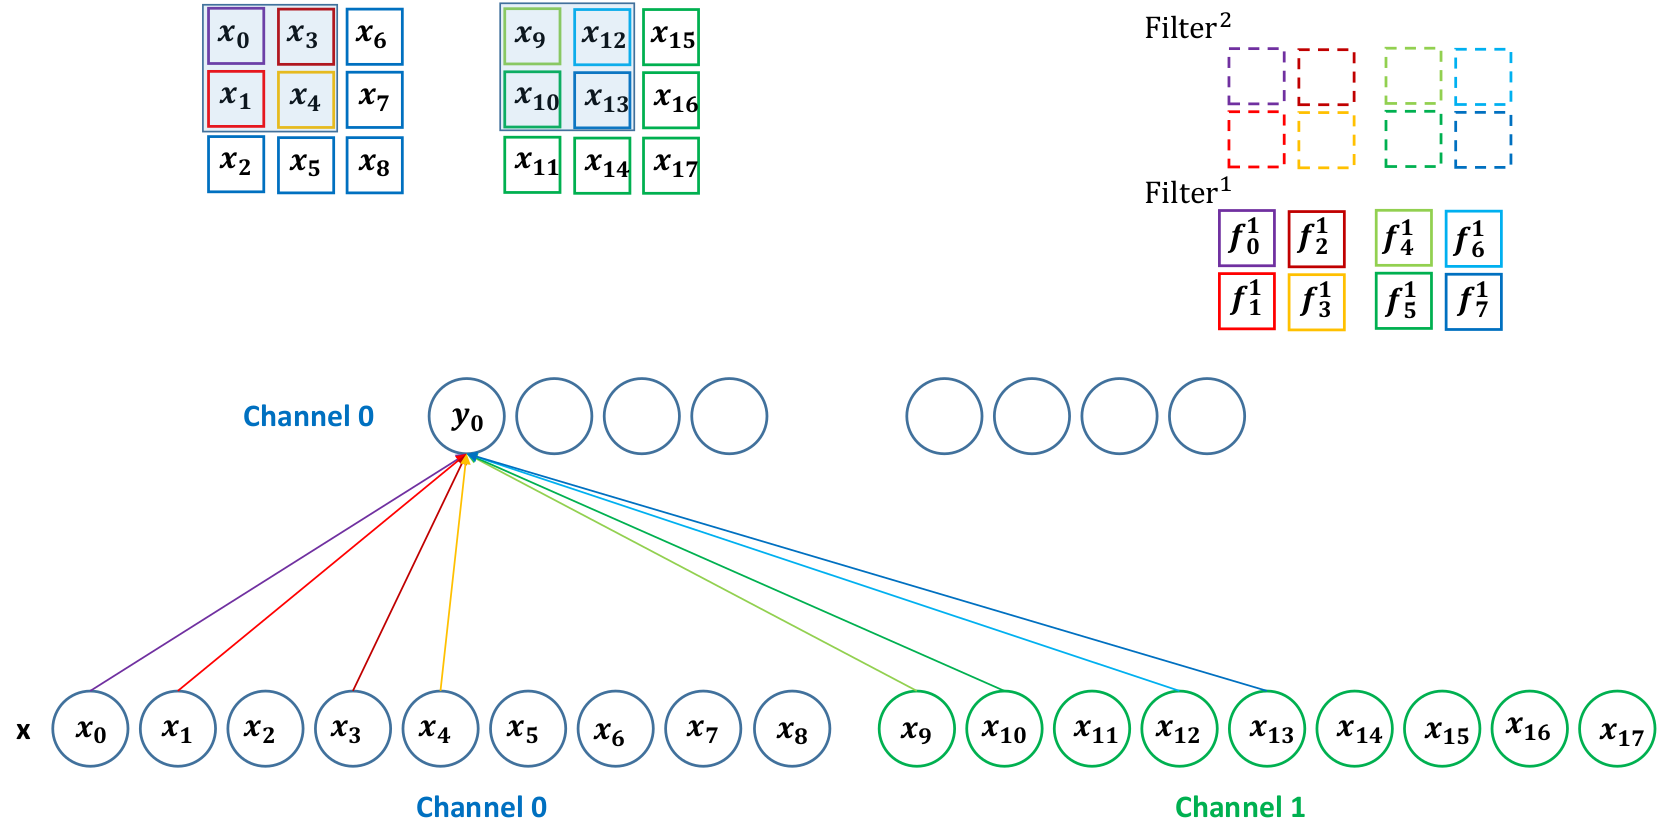
\includegraphics[width=\linewidth]{figures/convolution.png}
	$$Y = X * F + b$$
	\textbf{Backward-Pass} $*_F$ bezeichnet die Full-Convolution\\
	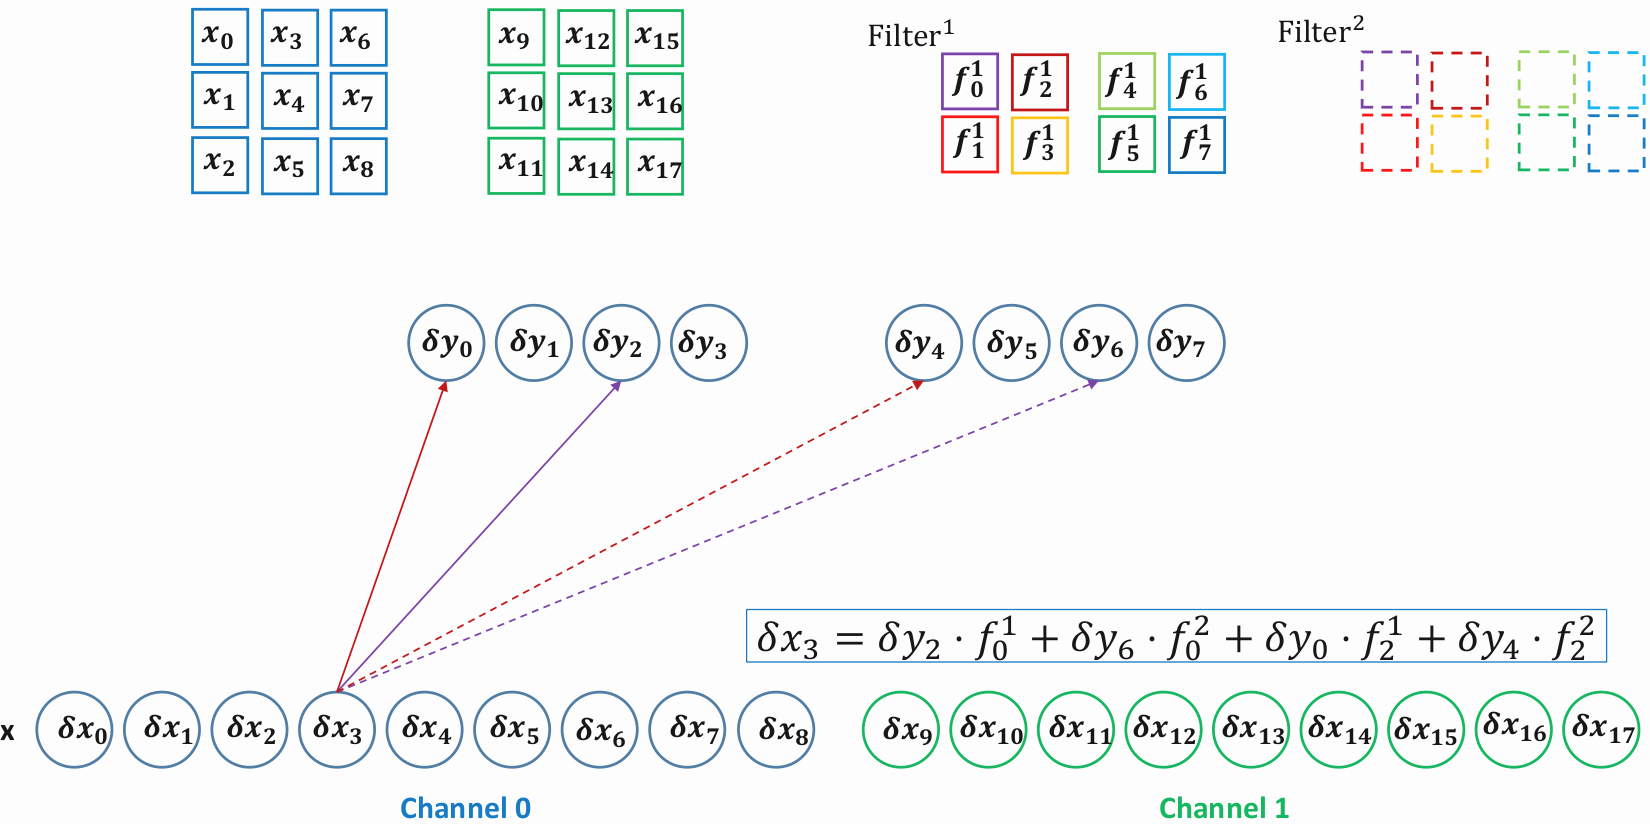
\includegraphics[width=\linewidth]{figures/convolution-backward.png}
	$$\delta X = \delta Y *_F rot^{180}_{h,w}(trans(F))$$
	\textbf{Calculate Delta Weights} $*_{ch}$ bezeichnet die Channel-Wise-Convolution, $f$ ist ein Element des Filtertensors
	$$\frac{\delta L}{\delta f} = X *_{ch} \delta Y$$
	$$\frac{\delta L}{\delta b_f} = \sum_i \delta y_{i,f}$$
	\subsection{Pooling}
	Reduziert die Werte innerhalb eines Filters auf einen Wert (z.B. Maximum oder Durchschnitt). Filter wird ohne Überlappung (mit Stride) verschoben.\\
	\textbf{Forward-Pass}\\
	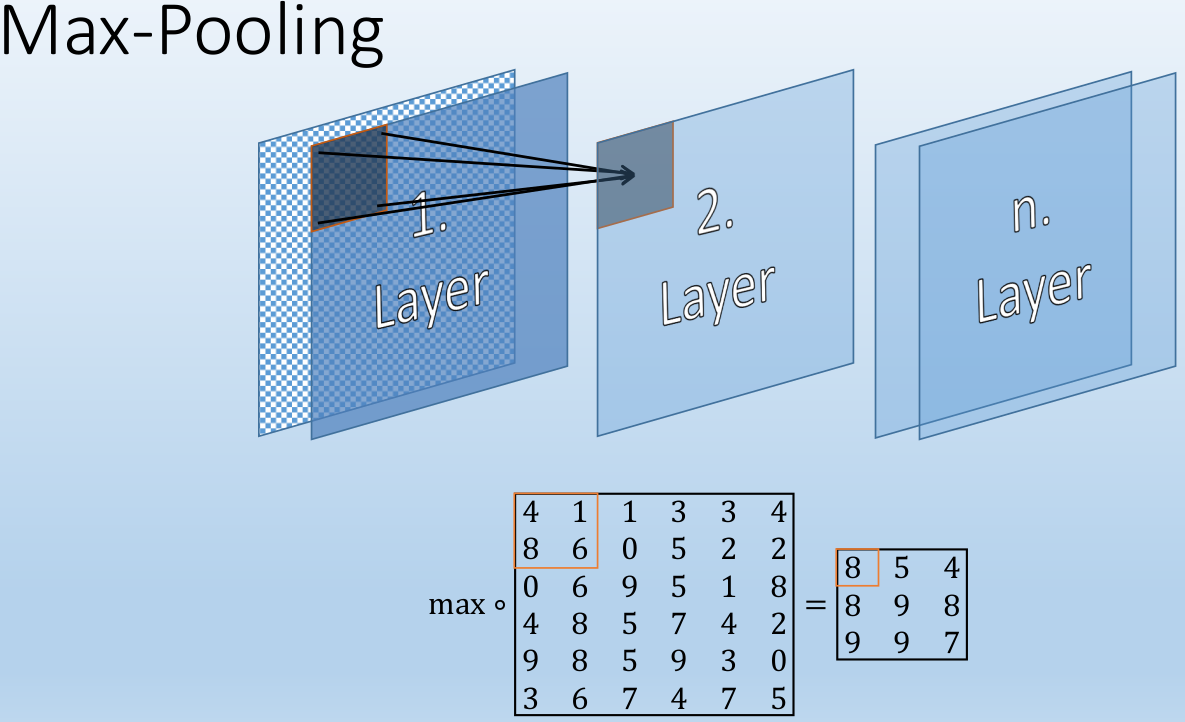
\includegraphics[width=\linewidth]{figures/max-pooling.png}\\
	\textbf{Backward-Pass} Nur die Elemente, die im Forward-Pass an der Berechnung des Outputs beteiligt waren, bekommen anteilig oder ganz das Delta des jeweiligen Outputs.
	$$\delta x_i = (x_i == max) ? \delta y : 0$$
	\subsection{Vanilla RNN}
	Recurrent Neuronal Networks (RNNs) werden verwendet, um Daten unterschiedlicher Länge zu verarbeiten. Dabei wird ein Hidden State $h$ in jedem Schritt um Informationen der Eingabe ergänzt.\\
	\textbf{Parameter}\\
	$[x_0, \cdots, x_n] = X \in \R^{n \times m}$: Eingabevektoren mit jeweils Länge $m$\\
	$g$: Zwischenvariable nach der Addition vor $\tanh$\\
	$h$: Hidden State ($h_{-1}$ kann mit Nullen initialisiert werden)\\
	$W_x, W_h, W_o$: Gewichtsmatrizen\\
	$b$: Bias\\
	$[o_0, \cdots, o_n] = O \in \R^{n \times l}$: Ausgabevektoren mit jeweils Länge $l$\\
	\textbf{Funktionsweise}\\
	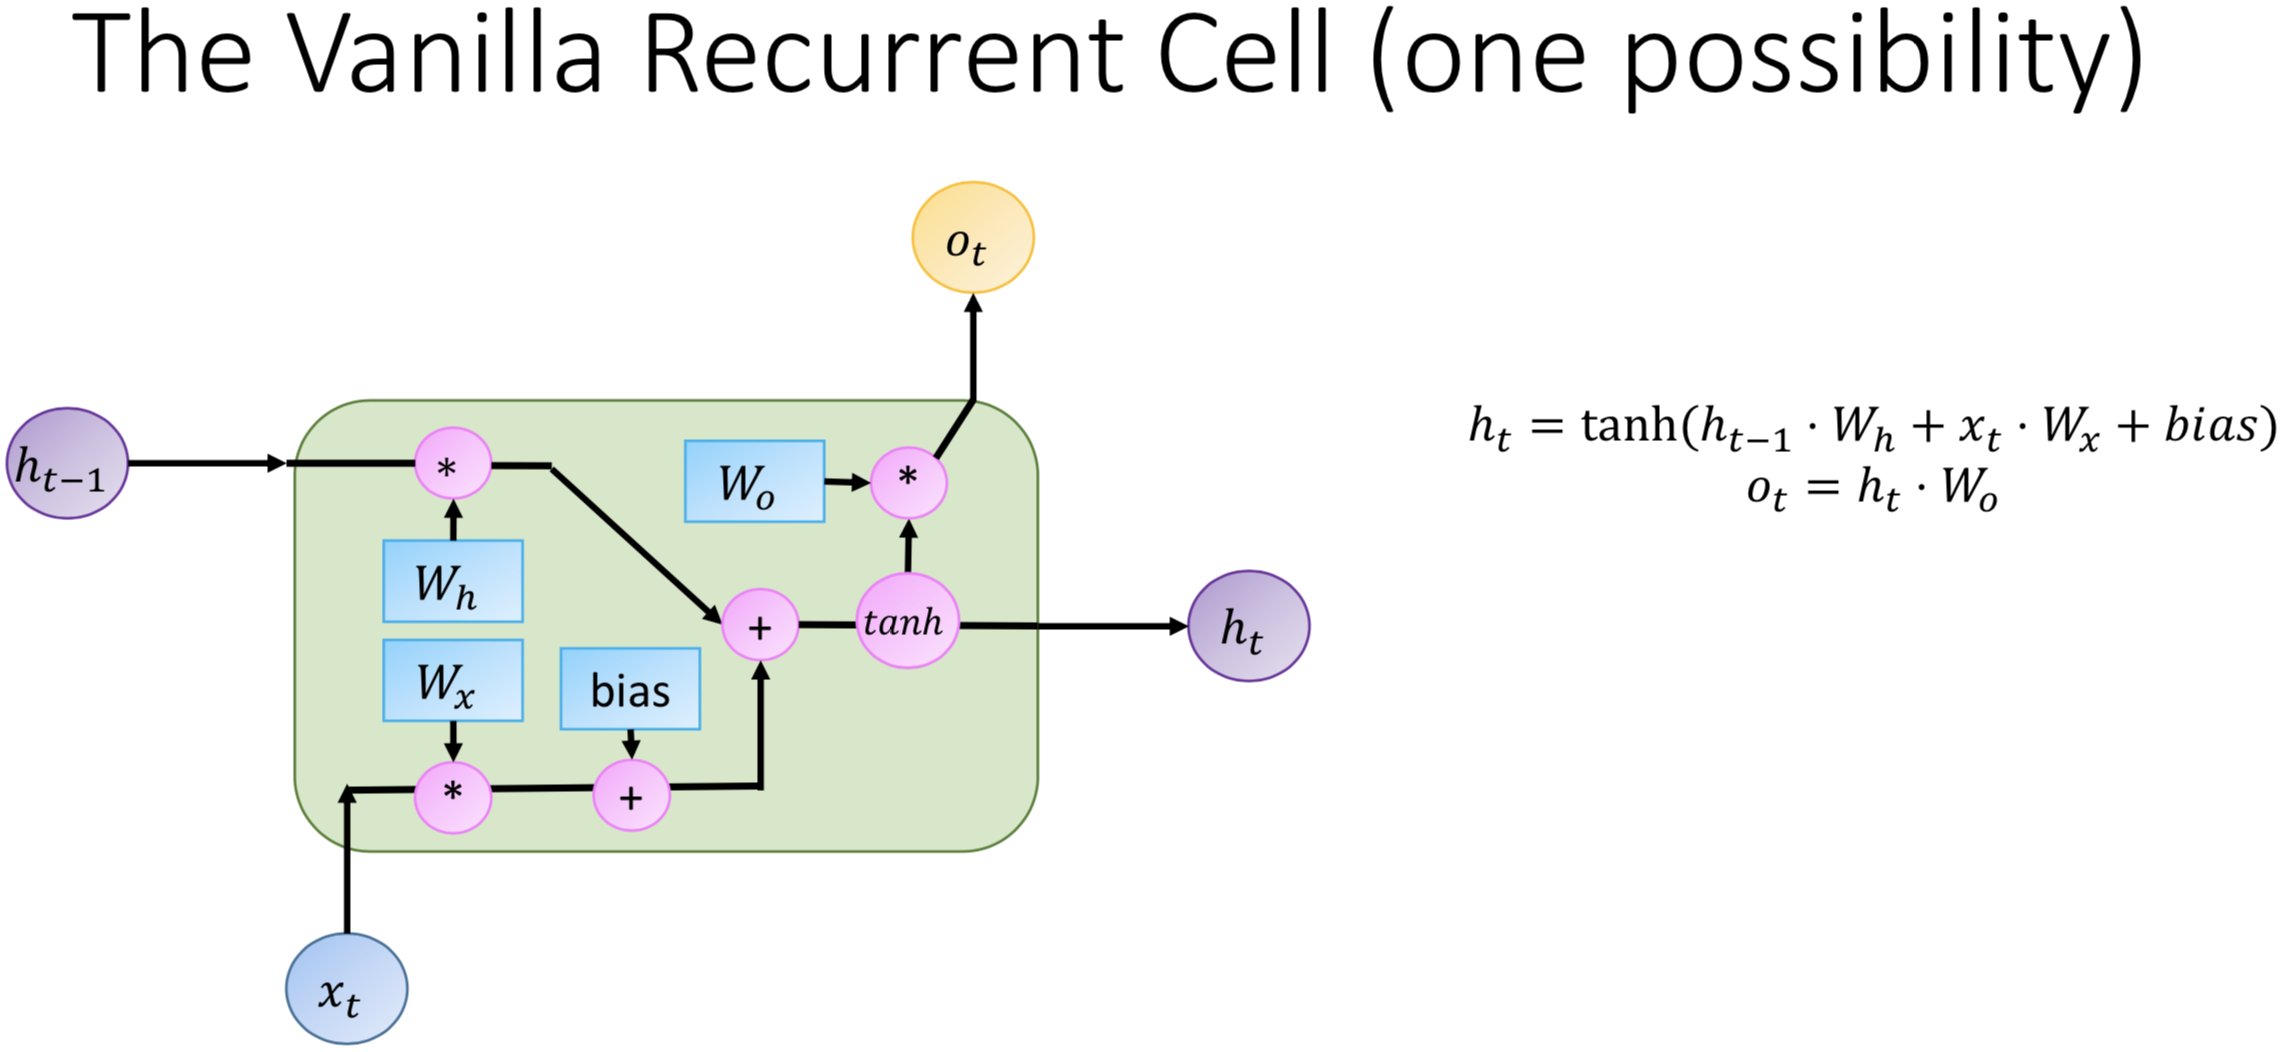
\includegraphics[width=\linewidth]{figures/vanilla-rnn.png}\\
	\textbf{Forward-Pass}
	$$h_t = \tanh(h_{t-1} \cdot W_h + x_t \cdot W_x + b)$$
	$$o_t = h_t \cdot W_o$$
	\textbf{Backward-Pass}
	$$\delta h_t = \delta o_t \cdot W_o^T + \delta g_{t+1} \cdot W_h^T$$
	$$\delta g_t = \delta h_t \cdot (1 - \tanh^2(g_t)) = \delta h_t \cdot (1 - h_t^2)$$
	$$\delta x_t = \delta g_t \cdot W_x^T$$
	\textbf{Calculate Delta Weights}
	$$\delta W_h = \sum_t h_{t-1}^T \cdot \delta g_t$$
	$$\delta W_x = \sum_t x_t^T \cdot \delta g_t$$
	$$\delta W_o = \sum_t h_t^T \cdot \delta o_t$$
	$$\delta b = \sum_t \delta g_t$$
	\subsection{Gru}
	Verwendet zwei Gates (wie $g$ im Vanilla RNN), um zu bestimmen, was aus dem alten Internal State $h$ übernommen wird und was von den aktuell verarbeiteten Daten hinzugefügt wird.\\
	\textbf{Funktionsweise}\\
	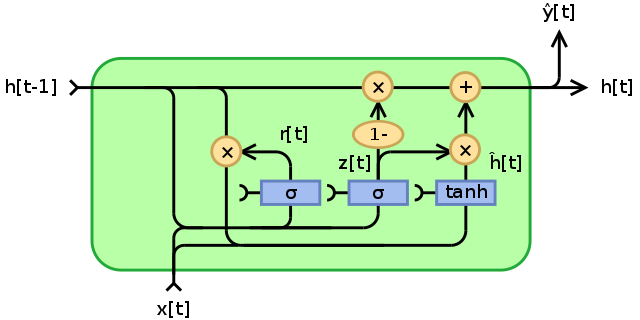
\includegraphics[width=\linewidth]{figures/gru.png}
	\subsection{LSTM}
	Verwendet drei Gates (Forget, Input, Output) und zusätzlichen State $c$\\
	\textbf{Funktionsweise}\\
	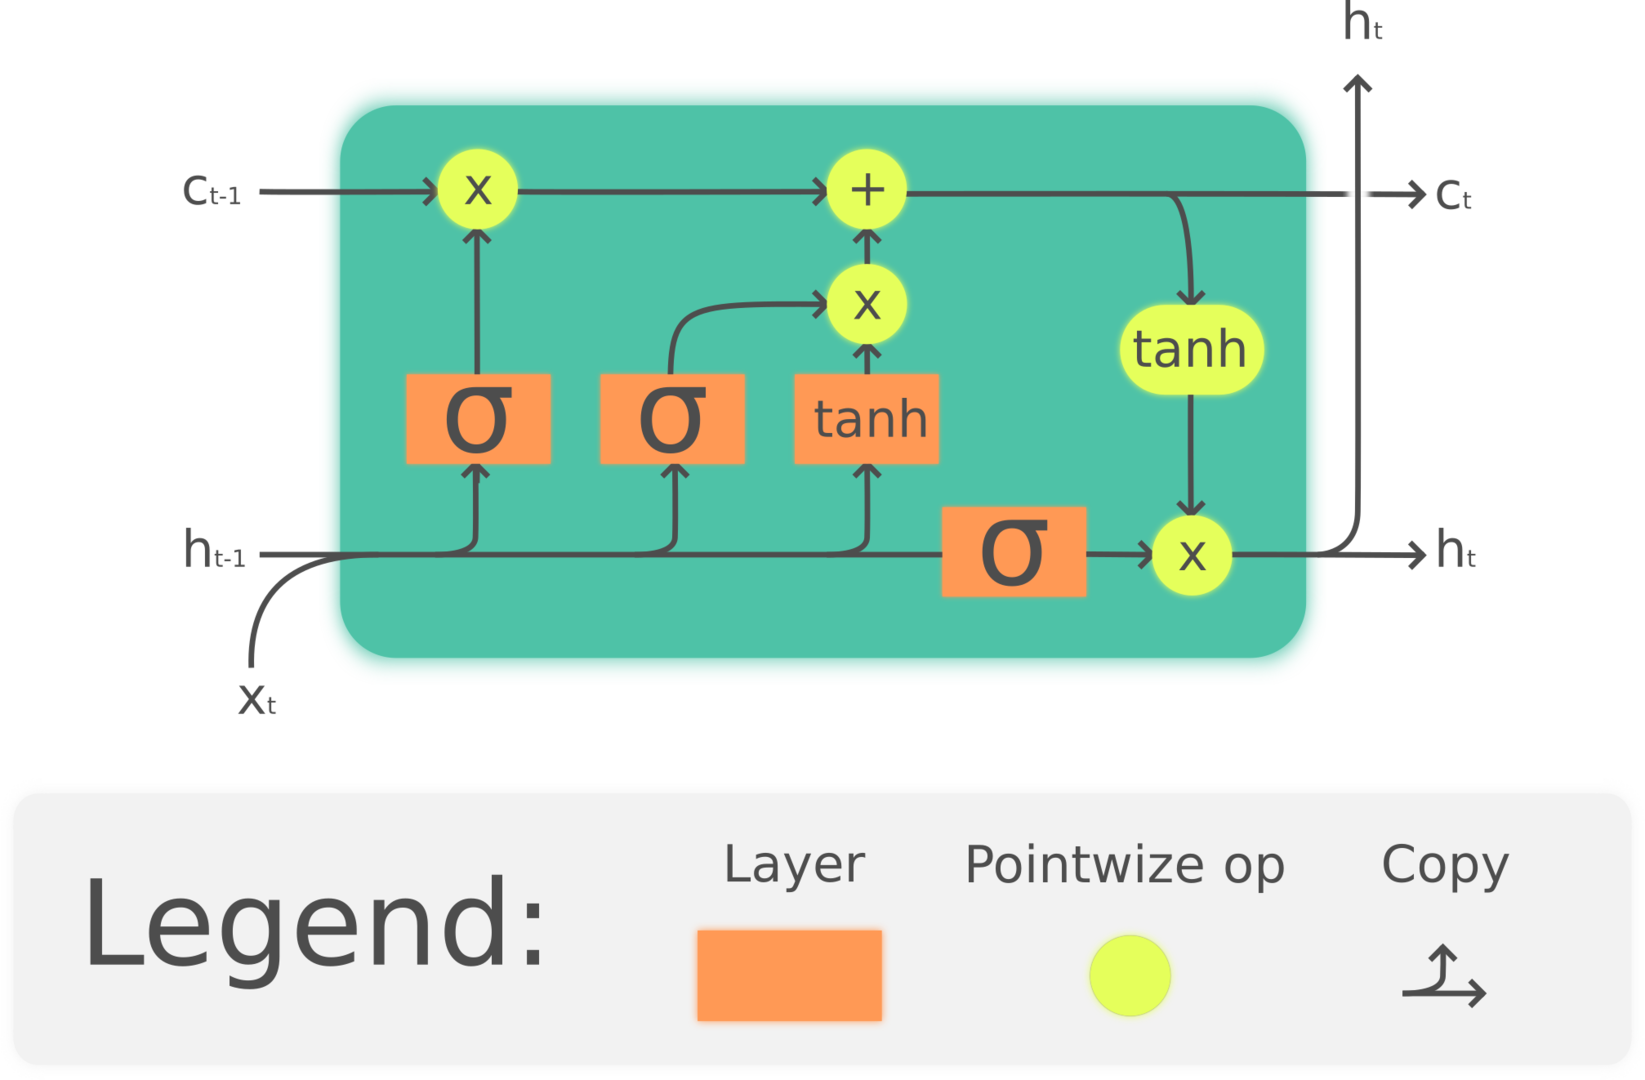
\includegraphics[width=\linewidth]{figures/lstm.png}
	\subsection{Highway Layer}
	Verwendet ein Gate, das bestimmt, ob der Layer wie ein Fully Connected Layer funktioniert oder lediglich den Input weitergibt. Wird verwendet bei sehr tiefen Netzwerken ($>$ 100 Layer), um Daten über lange Zeit/viele Layer hinweg nutzbar zu machen.\\
	\textbf{Forward-Pass}
	$$Y = (X \cdot W + b) \cdot T(x) + x \cdot (1 - T(x))$$
	$$T(x) = \sigma(x \cdot W_T + b_T)$$


	\section{Loss-Funktionen}
	$X$: Eingabe der Loss-Funktion bzw. Ausgabe des Netzes (Prediction)\\
	$T$: Erwartetes Ergebnis (Ground Truth)
	\subsection{Cross Entropy}
	Negative-Log-Likelihood, Cross-Entropy\\
	\textbf{Forward-Pass} $$L = -\sum_i t_i \cdot \log(x_i)$$
	\textbf{Backward-Pass} $$\frac{\delta L}{\delta x_i} = -\frac{t_i}{x_i}$$
	\subsection{Mean Squared Error}
	Euklidischer Loss, Mean-Squared-Error, $l_2$-Loss\\
	\textbf{Forward-Pass} $$L = \sum_i \frac{1}{2} (x_i - t_i)^2$$
	\textbf{Backward-Pass} $$\frac{\delta L}{\delta x_i} = t_i - x_i$$



	\section{aus KI2-Vorlesung}
	\textbf{Perceptron} (= künstliches Neuron) stellt lineare Trennung (binäre Klassifikation) dar. Kann Funktionen AND, OR und NOT lernen, nicht aber XOR.\\
	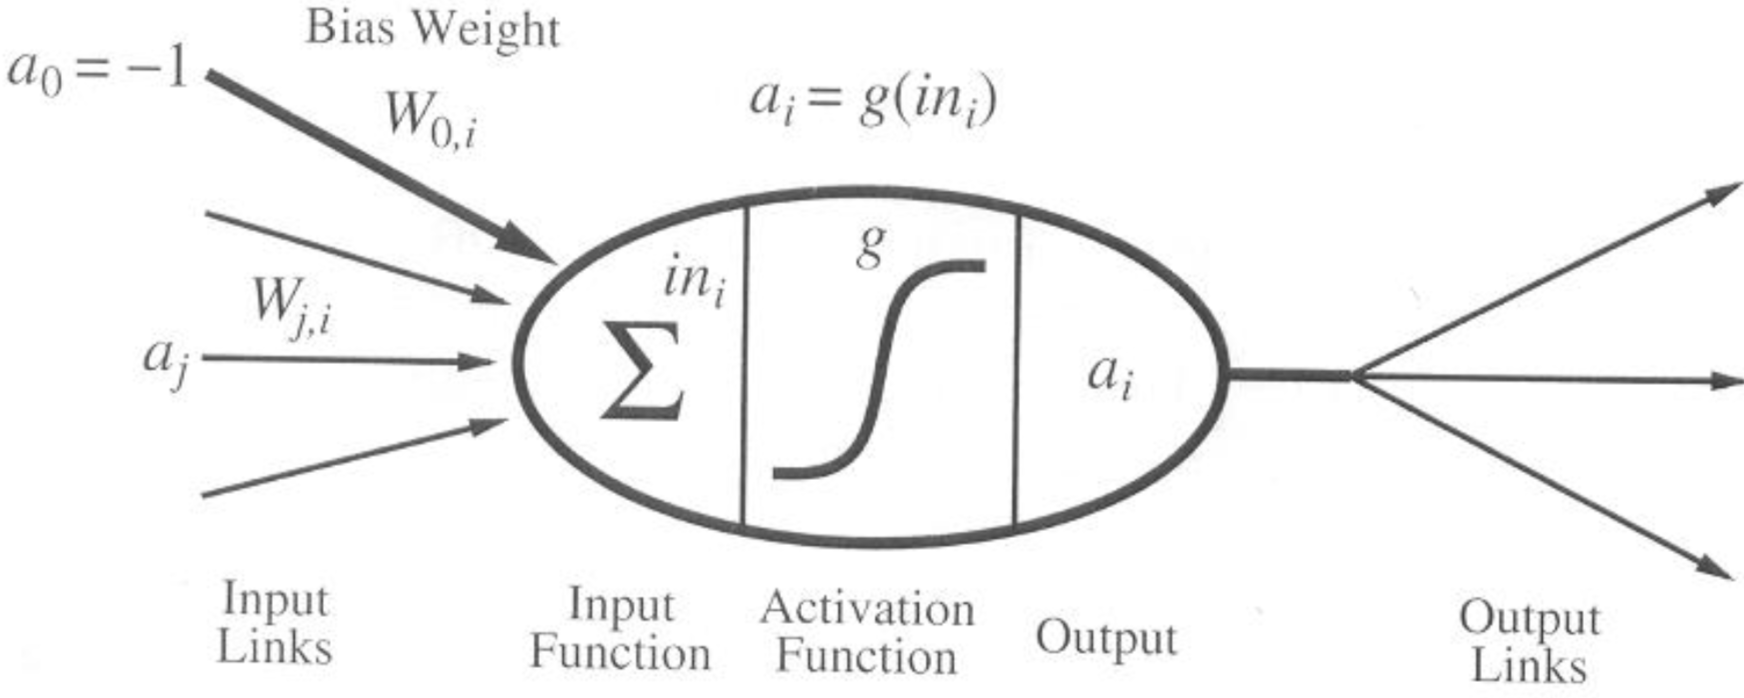
\includegraphics[width=\linewidth]{figures/perceptron.png}\\
	mit Inputs $a_j$ gewichtet mit $W_{ji}$ (ergeben zusammen die Gewichtsmatrix $W$), Outputs $a_i$ und der Aktivierungsfunktion $g$ mit der der Output berechnet wird.\\
	\textbf{Bias} ist der Input eines Perceptrons, der immer konstant bleibt (meist 1) damit das Perceptron auch bei schwachem Input nicht abgeschaltet wird.\\
	\textbf{Aktivierungsfunktionen} typisch sind:
	\begin{itemize}
		\item Stufenfunktion: $g(x) = x < 0 \rightarrow 0, x > 0 \rightarrow 1$ (nicht differenzierbar)
		\item Sigmoidfunktion: $g(x) = \frac{1}{1 + e^{-x}}$ (siehe Einleitung Lernen)
		\item ReLU (Rectified Linear Unit): $g(x) = x < 0 \rightarrow 0, x > 0 \rightarrow x$ (nicht differenzierbar für $x=0$)
		\item Tangenz hyperbolicus: $g(x) = tanh(x)$
		\item Softmax: Abbildung eines Vektors in Werte zwischen 0 und 1 mit Summe 1 (z.B. für Ausgabelayer)
	\end{itemize}
	\textbf{Loss-Funktion} Liefert einen Wert, der repräsentiert, wie gut ein neuronales Netz bereits trainiert ist. Wird anhand des Abgleichs von Vorhersage und tatsächlichem Wert (Ground Truth) berechnet.\\
	\textbf{Berechnung der Ausgabe}
	$$Ausgabe_{Schicht(x)} = g(W \cdot Eingabe_{Schicht(x)}) = Eingabe_{Schicht(x+1)}$$
	\textbf{Rückpropagierung} Fehler (z.B. quadratische Abweichung von erwartetem Wert $\rightarrow$ Loss-Funktion) wird entsprechend der Gewichte auf Vorgängerknoten verteilt\\
	\textbf{Verteilung des Fehlers}
	$$Fehler_{Schicht(x-1)} = W^T \cdot Fehler_{Schicht(x)}$$
	Änderung der Gewichte über Gradient Descent $w_{jk} \leftarrow w_{jk} - \alpha \frac{dE}{dw_{jk}}$ mit $E$ als Loss-Funktion\\
	\textbf{Datenvorverarbeitung} Inputs zwischen 0 und 1, da hohe Werte niedrige Gradienten erzeugen, Bilder können rotiert, gespiegelt, zugeschnitten, etc. werden um mehr Trainingsdaten zu generieren.\\
	\textbf{Netzvorbereitung} zufällige Vorbelegung der Gewichte (nicht symmetrisch) $\Rightarrow$ Pre-Training: wenn möglich Gewichte eines bereits trainierten Netzes für ähnliches Problem verwenden\\
	\textbf{Overfitting} kann durch kleine Netzgröße (nicht so ausdrucksstark), Dropout (ignorieren einiger Knoten für einen Lerndurchgang)\\
	\textbf{Typen von Schichten}
	\begin{itemize}
		\item Fully Connected (FC): besteht aus mehreren Perceptrons (s.o.)
		\item Convolutional Neural Networks (CNN): Für Bilderkennung, Gewichtungsmatrix über Input verschieben und gewichtete, aufsummierte Werte in Outputmatrix schreiben
		\item Polling Layer: Verkleinerung von Inputmatrizen durch z.B. Max-Funktion einer Submatrix
	\end{itemize}
	\textbf{Multi-Klassen Klassifizierung} über $K$ Diskrimianzfunktionen für $K$ Klassen. Dabei gibt immer eine Funktion für einen bestimmten Bereich/Klasse den höchsten Wert zurück.\\
	\textbf{Vanishing Problem} Tiefe Netze lernen sehr langsam, da das Änderungsgewicht pro Schicht mit Faktor < 1 multipliziert wird (Ableitung Aktivierungsfunktion). Kann umgangen werden durch ReLU (Ableitung konstant 1 für positive Zahlen)\\
	\textbf{Recurrent Neural Networks} für die Verarbeitung von sequenziellen Daten (variable Ein-/Ausgabe) z.B. für OCR oder Sprachverarbeitung\\
	\textbf{Adversial Examples} Manipulierte Inputdaten, die für den Menschen noch gut erkennbar sind (kein merklicher Unterschied zu Original), von einem DNN jedoch falsch klassifiziert werden. Bild wird mit Rauschen addiert, welches auf das Netz trainiert ist. Gegenmaßnahmen:
	\begin{itemize}
		\item Trainiere Netz mit Adversial Examples (richtige Klassifikation)
		\item Mehrere unterschiedliche Technologien zur Klassifikation einsetzen
		\item DeepCloak entfernen von unnötigen Features, die ausgenutzt werden könnten
	\end{itemize}
	
\end{document}
